% Created by tikzDevice version 0.12.6 on 2025-01-28 09:53:46
% !TEX encoding = UTF-8 Unicode
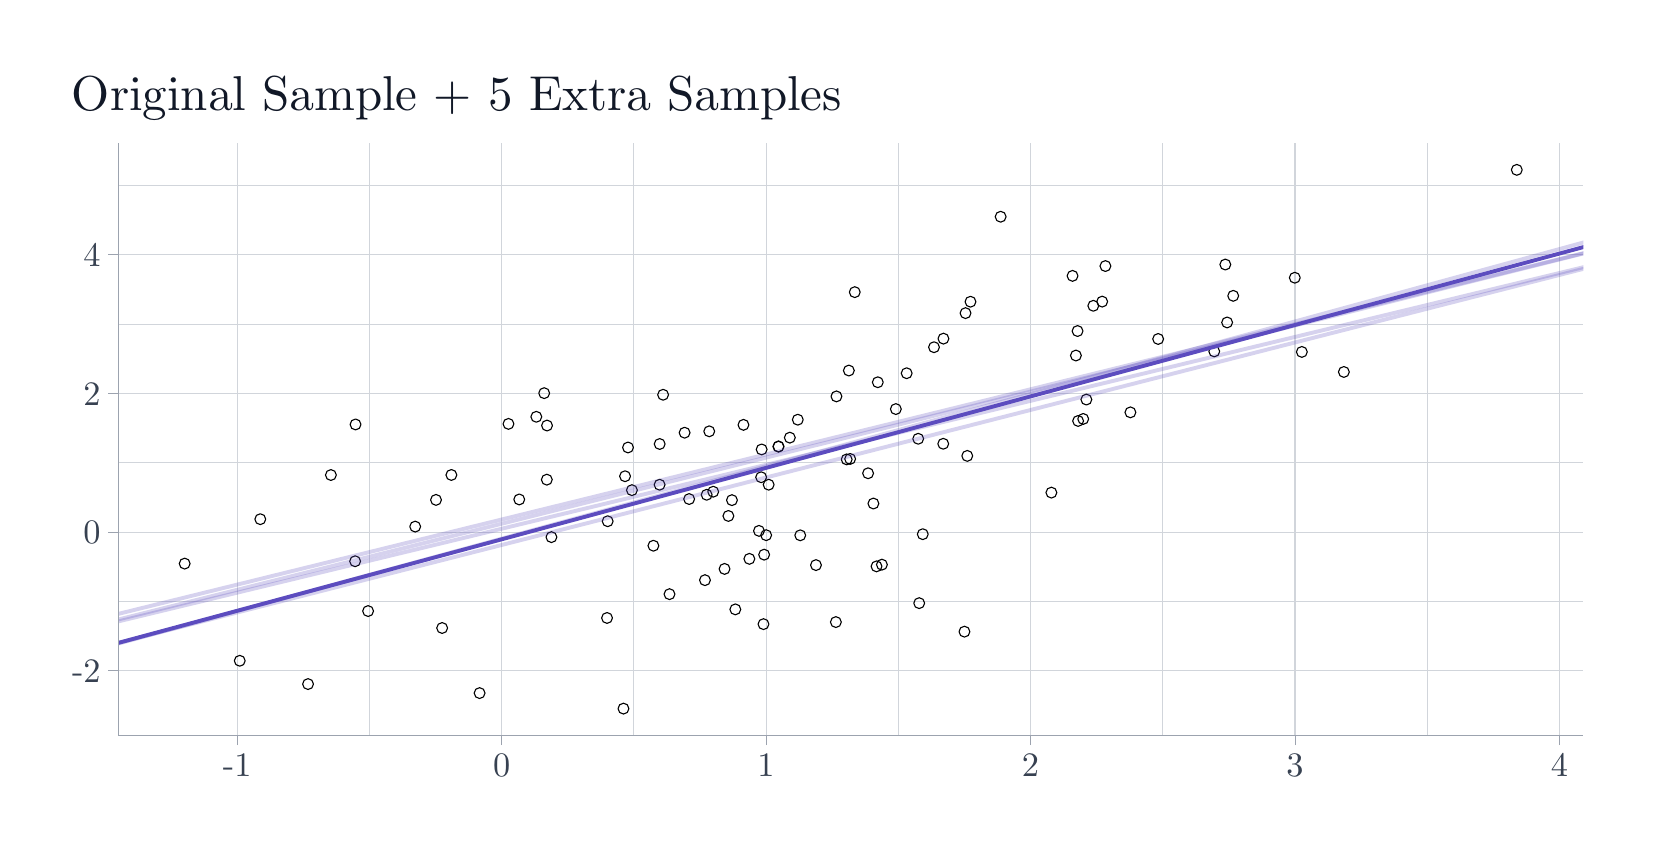
\begin{tikzpicture}[x=1pt,y=1pt]
\definecolor{fillColor}{RGB}{255,255,255}
\path[use as bounding box,fill=fillColor] (0,0) rectangle (578.16,289.08);
\begin{scope}
\path[clip] (  0.00,  0.00) rectangle (578.16,289.08);
\definecolor{drawColor}{RGB}{255,255,255}

\path[draw=drawColor,line width= 0.7pt,line join=round,line cap=round,fill=fillColor] ( -0.00,  0.00) rectangle (578.16,289.08);
\end{scope}
\begin{scope}
\path[clip] ( 32.66, 33.29) rectangle (562.16,247.43);
\definecolor{drawColor}{RGB}{255,255,255}
\definecolor{fillColor}{RGB}{255,255,255}

\path[draw=drawColor,line width= 0.7pt,line join=round,line cap=round,fill=fillColor] ( 32.66, 33.29) rectangle (562.16,247.43);
\definecolor{drawColor}{RGB}{209,213,219}

\path[draw=drawColor,line width= 0.4pt,line join=round] ( 32.66, 81.75) --
	(562.16, 81.75);

\path[draw=drawColor,line width= 0.4pt,line join=round] ( 32.66,131.86) --
	(562.16,131.86);

\path[draw=drawColor,line width= 0.4pt,line join=round] ( 32.66,181.97) --
	(562.16,181.97);

\path[draw=drawColor,line width= 0.4pt,line join=round] ( 32.66,232.09) --
	(562.16,232.09);

\path[draw=drawColor,line width= 0.4pt,line join=round] (123.47, 33.29) --
	(123.47,247.43);

\path[draw=drawColor,line width= 0.4pt,line join=round] (219.03, 33.29) --
	(219.03,247.43);

\path[draw=drawColor,line width= 0.4pt,line join=round] (314.60, 33.29) --
	(314.60,247.43);

\path[draw=drawColor,line width= 0.4pt,line join=round] (410.16, 33.29) --
	(410.16,247.43);

\path[draw=drawColor,line width= 0.4pt,line join=round] (505.72, 33.29) --
	(505.72,247.43);

\path[draw=drawColor,line width= 0.4pt,line join=round] ( 32.66, 56.69) --
	(562.16, 56.69);

\path[draw=drawColor,line width= 0.4pt,line join=round] ( 32.66,106.81) --
	(562.16,106.81);

\path[draw=drawColor,line width= 0.4pt,line join=round] ( 32.66,156.92) --
	(562.16,156.92);

\path[draw=drawColor,line width= 0.4pt,line join=round] ( 32.66,207.03) --
	(562.16,207.03);

\path[draw=drawColor,line width= 0.4pt,line join=round] ( 75.69, 33.29) --
	( 75.69,247.43);

\path[draw=drawColor,line width= 0.4pt,line join=round] (171.25, 33.29) --
	(171.25,247.43);

\path[draw=drawColor,line width= 0.4pt,line join=round] (266.81, 33.29) --
	(266.81,247.43);

\path[draw=drawColor,line width= 0.4pt,line join=round] (362.38, 33.29) --
	(362.38,247.43);

\path[draw=drawColor,line width= 0.4pt,line join=round] (457.94, 33.29) --
	(457.94,247.43);

\path[draw=drawColor,line width= 0.4pt,line join=round] (553.50, 33.29) --
	(553.50,247.43);
\definecolor{drawColor}{RGB}{0,0,0}

\path[draw=drawColor,line width= 0.4pt,line join=round,line cap=round] (432.77,203.49) circle (  1.96);

\path[draw=drawColor,line width= 0.4pt,line join=round,line cap=round] (123.01, 78.27) circle (  1.96);

\path[draw=drawColor,line width= 0.4pt,line join=round,line cap=round] (435.62,192.18) circle (  1.96);

\path[draw=drawColor,line width= 0.4pt,line join=round,line cap=round] (246.28,143.22) circle (  1.96);

\path[draw=drawColor,line width= 0.4pt,line join=round,line cap=round] (177.63,118.60) circle (  1.96);

\path[draw=drawColor,line width= 0.4pt,line join=round,line cap=round] (379.37,179.46) circle (  1.96);

\path[draw=drawColor,line width= 0.4pt,line join=round,line cap=round] (153.11,127.45) circle (  1.96);

\path[draw=drawColor,line width= 0.4pt,line join=round,line cap=round] (253.20,112.64) circle (  1.96);

\path[draw=drawColor,line width= 0.4pt,line join=round,line cap=round] (266.12, 98.65) circle (  1.96);

\path[draw=drawColor,line width= 0.4pt,line join=round,line cap=round] (228.37,138.64) circle (  1.96);

\path[draw=drawColor,line width= 0.4pt,line join=round,line cap=round] (279.17,105.64) circle (  1.96);

\path[draw=drawColor,line width= 0.4pt,line join=round,line cap=round] (251.81, 93.50) circle (  1.96);

\path[draw=drawColor,line width= 0.4pt,line join=round,line cap=round] (187.59,125.75) circle (  1.96);

\path[draw=drawColor,line width= 0.4pt,line join=round,line cap=round] (260.78, 97.14) circle (  1.96);

\path[draw=drawColor,line width= 0.4pt,line join=round,line cap=round] (237.38,142.72) circle (  1.96);

\path[draw=drawColor,line width= 0.4pt,line join=round,line cap=round] (369.92,121.07) circle (  1.96);

\path[draw=drawColor,line width= 0.4pt,line join=round,line cap=round] (303.68,128.06) circle (  1.96);

\path[draw=drawColor,line width= 0.4pt,line join=round,line cap=round] (327.50,173.61) circle (  1.96);

\path[draw=drawColor,line width= 0.4pt,line join=round,line cap=round] (183.80,148.47) circle (  1.96);

\path[draw=drawColor,line width= 0.4pt,line join=round,line cap=round] (118.47,145.70) circle (  1.96);

\path[draw=drawColor,line width= 0.4pt,line join=round,line cap=round] (379.57,146.97) circle (  1.96);

\path[draw=drawColor,line width= 0.4pt,line join=round,line cap=round] (460.42,171.91) circle (  1.96);

\path[draw=drawColor,line width= 0.4pt,line join=round,line cap=round] (109.57,127.43) circle (  1.96);

\path[draw=drawColor,line width= 0.4pt,line join=round,line cap=round] (307.19,160.95) circle (  1.96);

\path[draw=drawColor,line width= 0.4pt,line join=round,line cap=round] (265.88, 73.55) circle (  1.96);

\path[draw=drawColor,line width= 0.4pt,line join=round,line cap=round] (428.77,172.09) circle (  1.96);

\path[draw=drawColor,line width= 0.4pt,line join=round,line cap=round] (209.58,110.73) circle (  1.96);

\path[draw=drawColor,line width= 0.4pt,line join=round,line cap=round] (389.44,202.94) circle (  1.96);

\path[draw=drawColor,line width= 0.4pt,line join=round,line cap=round] (189.26,104.99) circle (  1.96);

\path[draw=drawColor,line width= 0.4pt,line join=round,line cap=round] (258.65,145.56) circle (  1.96);

\path[draw=drawColor,line width= 0.4pt,line join=round,line cap=round] (330.84,138.72) circle (  1.96);

\path[draw=drawColor,line width= 0.4pt,line join=round,line cap=round] ( 76.63, 60.31) circle (  1.96);

\path[draw=drawColor,line width= 0.4pt,line join=round,line cap=round] (231.92, 84.38) circle (  1.96);

\path[draw=drawColor,line width= 0.4pt,line join=round,line cap=round] (308.68, 95.04) circle (  1.96);

\path[draw=drawColor,line width= 0.4pt,line join=round,line cap=round] (101.31, 51.89) circle (  1.96);

\path[draw=drawColor,line width= 0.4pt,line join=round,line cap=round] (338.89,185.93) circle (  1.96);

\path[draw=drawColor,line width= 0.4pt,line join=round,line cap=round] (292.04, 74.29) circle (  1.96);

\path[draw=drawColor,line width= 0.4pt,line join=round,line cap=round] (216.93,137.38) circle (  1.96);

\path[draw=drawColor,line width= 0.4pt,line join=round,line cap=round] (305.61,117.13) circle (  1.96);

\path[draw=drawColor,line width= 0.4pt,line join=round,line cap=round] (381.42,147.69) circle (  1.96);

\path[draw=drawColor,line width= 0.4pt,line join=round,line cap=round] (149.77, 72.15) circle (  1.96);

\path[draw=drawColor,line width= 0.4pt,line join=round,line cap=round] (457.87,198.72) circle (  1.96);

\path[draw=drawColor,line width= 0.4pt,line join=round,line cap=round] (340.68,190.05) circle (  1.96);

\path[draw=drawColor,line width= 0.4pt,line join=round,line cap=round] (255.71, 78.88) circle (  1.96);

\path[draw=drawColor,line width= 0.4pt,line join=round,line cap=round] (265.22,136.67) circle (  1.96);

\path[draw=drawColor,line width= 0.4pt,line join=round,line cap=round] (378.78,170.61) circle (  1.96);

\path[draw=drawColor,line width= 0.4pt,line join=round,line cap=round] (239.02,118.75) circle (  1.96);

\path[draw=drawColor,line width= 0.4pt,line join=round,line cap=round] (186.64,157.01) circle (  1.96);

\path[draw=drawColor,line width= 0.4pt,line join=round,line cap=round] (382.56,154.70) circle (  1.96);

\path[draw=drawColor,line width= 0.4pt,line join=round,line cap=round] (187.67,145.31) circle (  1.96);

\path[draw=drawColor,line width= 0.4pt,line join=round,line cap=round] (209.35, 75.78) circle (  1.96);

\path[draw=drawColor,line width= 0.4pt,line join=round,line cap=round] (377.56,199.39) circle (  1.96);

\path[draw=drawColor,line width= 0.4pt,line join=round,line cap=round] (408.50,176.59) circle (  1.96);

\path[draw=drawColor,line width= 0.4pt,line join=round,line cap=round] (140.03,108.79) circle (  1.96);

\path[draw=drawColor,line width= 0.4pt,line join=round,line cap=round] ( 56.73, 95.42) circle (  1.96);

\path[draw=drawColor,line width= 0.4pt,line join=round,line cap=round] (475.60,164.67) circle (  1.96);

\path[draw=drawColor,line width= 0.4pt,line join=round,line cap=round] (339.52,134.34) circle (  1.96);

\path[draw=drawColor,line width= 0.4pt,line join=round,line cap=round] (163.30, 48.63) circle (  1.96);

\path[draw=drawColor,line width= 0.4pt,line join=round,line cap=round] (228.34,123.92) circle (  1.96);

\path[draw=drawColor,line width= 0.4pt,line join=round,line cap=round] (173.73,145.91) circle (  1.96);

\path[draw=drawColor,line width= 0.4pt,line join=round,line cap=round] (271.32,137.76) circle (  1.96);

\path[draw=drawColor,line width= 0.4pt,line join=round,line cap=round] (278.28,147.42) circle (  1.96);

\path[draw=drawColor,line width= 0.4pt,line join=round,line cap=round] (388.27,190.09) circle (  1.96);

\path[draw=drawColor,line width= 0.4pt,line join=round,line cap=round] (322.15, 81.13) circle (  1.96);

\path[draw=drawColor,line width= 0.4pt,line join=round,line cap=round] (245.35,120.29) circle (  1.96);

\path[draw=drawColor,line width= 0.4pt,line join=round,line cap=round] (229.61,156.43) circle (  1.96);

\path[draw=drawColor,line width= 0.4pt,line join=round,line cap=round] (247.72,121.40) circle (  1.96);

\path[draw=drawColor,line width= 0.4pt,line join=round,line cap=round] (323.44,106.05) circle (  1.96);

\path[draw=drawColor,line width= 0.4pt,line join=round,line cap=round] (226.11,101.88) circle (  1.96);

\path[draw=drawColor,line width= 0.4pt,line join=round,line cap=round] (330.91,176.71) circle (  1.96);

\path[draw=drawColor,line width= 0.4pt,line join=round,line cap=round] (351.58,220.76) circle (  1.96);

\path[draw=drawColor,line width= 0.4pt,line join=round,line cap=round] (398.47,150.07) circle (  1.96);

\path[draw=drawColor,line width= 0.4pt,line join=round,line cap=round] (538.09,237.70) circle (  1.96);

\path[draw=drawColor,line width= 0.4pt,line join=round,line cap=round] (284.85, 94.88) circle (  1.96);

\path[draw=drawColor,line width= 0.4pt,line join=round,line cap=round] (385.07,188.58) circle (  1.96);

\path[draw=drawColor,line width= 0.4pt,line join=round,line cap=round] (295.95,133.07) circle (  1.96);

\path[draw=drawColor,line width= 0.4pt,line join=round,line cap=round] (147.55,118.44) circle (  1.96);

\path[draw=drawColor,line width= 0.4pt,line join=round,line cap=round] (298.87,193.51) circle (  1.96);

\path[draw=drawColor,line width= 0.4pt,line join=round,line cap=round] (218.34,121.96) circle (  1.96);

\path[draw=drawColor,line width= 0.4pt,line join=round,line cap=round] (338.50, 70.83) circle (  1.96);

\path[draw=drawColor,line width= 0.4pt,line join=round,line cap=round] (306.73, 94.42) circle (  1.96);

\path[draw=drawColor,line width= 0.4pt,line join=round,line cap=round] (297.20,133.24) circle (  1.96);

\path[draw=drawColor,line width= 0.4pt,line join=round,line cap=round] (313.71,151.26) circle (  1.96);

\path[draw=drawColor,line width= 0.4pt,line join=round,line cap=round] (266.85,105.69) circle (  1.96);

\path[draw=drawColor,line width= 0.4pt,line join=round,line cap=round] ( 84.06,111.47) circle (  1.96);

\path[draw=drawColor,line width= 0.4pt,line join=round,line cap=round] (317.62,164.21) circle (  1.96);

\path[draw=drawColor,line width= 0.4pt,line join=round,line cap=round] (244.74, 89.44) circle (  1.96);

\path[draw=drawColor,line width= 0.4pt,line join=round,line cap=round] (321.79,140.53) circle (  1.96);

\path[draw=drawColor,line width= 0.4pt,line join=round,line cap=round] (264.25,107.25) circle (  1.96);

\path[draw=drawColor,line width= 0.4pt,line join=round,line cap=round] (265.04,126.63) circle (  1.96);

\path[draw=drawColor,line width= 0.4pt,line join=round,line cap=round] (118.32, 96.27) circle (  1.96);

\path[draw=drawColor,line width= 0.4pt,line join=round,line cap=round] (215.29, 43.02) circle (  1.96);

\path[draw=drawColor,line width= 0.4pt,line join=round,line cap=round] (433.42,182.56) circle (  1.96);

\path[draw=drawColor,line width= 0.4pt,line join=round,line cap=round] (271.28,137.68) circle (  1.96);

\path[draw=drawColor,line width= 0.4pt,line join=round,line cap=round] (275.40,140.93) circle (  1.96);

\path[draw=drawColor,line width= 0.4pt,line join=round,line cap=round] (296.73,165.18) circle (  1.96);

\path[draw=drawColor,line width= 0.4pt,line join=round,line cap=round] (215.86,126.99) circle (  1.96);

\path[draw=drawColor,line width= 0.4pt,line join=round,line cap=round] (254.49,118.35) circle (  1.96);

\path[draw=drawColor,line width= 0.4pt,line join=round,line cap=round] (267.75,123.93) circle (  1.96);

\path[draw=drawColor,line width= 0.4pt,line join=round,line cap=round] (292.25,155.84) circle (  1.96);
\definecolor{drawColor}{RGB}{92,76,191}

\path[draw=drawColor,line width= 1.4pt,line join=round] (-496.83,-76.30) -- (1091.66,352.84);
\definecolor{drawColor}{RGB}{92,76,191}

\path[draw=drawColor,draw opacity=0.25,line width= 1.4pt,line join=round] (-496.83,-53.14) -- (1091.66,337.97);

\path[draw=drawColor,draw opacity=0.25,line width= 1.4pt,line join=round] (-496.83,-53.51) -- (1091.66,330.54);

\path[draw=drawColor,draw opacity=0.25,line width= 1.4pt,line join=round] (-496.83,-78.48) -- (1091.66,356.42);

\path[draw=drawColor,draw opacity=0.25,line width= 1.4pt,line join=round] (-496.83,-68.40) -- (1091.66,337.09);

\path[draw=drawColor,draw opacity=0.25,line width= 1.4pt,line join=round] (-496.83,-57.07) -- (1091.66,339.76);
\end{scope}
\begin{scope}
\path[clip] (  0.00,  0.00) rectangle (578.16,289.08);
\definecolor{drawColor}{RGB}{156,163,175}

\path[draw=drawColor,line width= 0.3pt,line join=round] ( 32.66, 33.29) --
	( 32.66,247.43);
\end{scope}
\begin{scope}
\path[clip] (  0.00,  0.00) rectangle (578.16,289.08);
\definecolor{drawColor}{RGB}{55,65,81}

\node[text=drawColor,anchor=base east,inner sep=0pt, outer sep=0pt, scale=  1.24] at ( 26.36, 52.41) {-2};

\node[text=drawColor,anchor=base east,inner sep=0pt, outer sep=0pt, scale=  1.24] at ( 26.36,102.52) {0};

\node[text=drawColor,anchor=base east,inner sep=0pt, outer sep=0pt, scale=  1.24] at ( 26.36,152.63) {2};

\node[text=drawColor,anchor=base east,inner sep=0pt, outer sep=0pt, scale=  1.24] at ( 26.36,202.75) {4};
\end{scope}
\begin{scope}
\path[clip] (  0.00,  0.00) rectangle (578.16,289.08);
\definecolor{drawColor}{RGB}{156,163,175}

\path[draw=drawColor,line width= 0.3pt,line join=round] ( 29.16, 56.69) --
	( 32.66, 56.69);

\path[draw=drawColor,line width= 0.3pt,line join=round] ( 29.16,106.81) --
	( 32.66,106.81);

\path[draw=drawColor,line width= 0.3pt,line join=round] ( 29.16,156.92) --
	( 32.66,156.92);

\path[draw=drawColor,line width= 0.3pt,line join=round] ( 29.16,207.03) --
	( 32.66,207.03);
\end{scope}
\begin{scope}
\path[clip] (  0.00,  0.00) rectangle (578.16,289.08);
\definecolor{drawColor}{RGB}{156,163,175}

\path[draw=drawColor,line width= 0.3pt,line join=round] ( 32.66, 33.29) --
	(562.16, 33.29);
\end{scope}
\begin{scope}
\path[clip] (  0.00,  0.00) rectangle (578.16,289.08);
\definecolor{drawColor}{RGB}{156,163,175}

\path[draw=drawColor,line width= 0.3pt,line join=round] ( 75.69, 29.79) --
	( 75.69, 33.29);

\path[draw=drawColor,line width= 0.3pt,line join=round] (171.25, 29.79) --
	(171.25, 33.29);

\path[draw=drawColor,line width= 0.3pt,line join=round] (266.81, 29.79) --
	(266.81, 33.29);

\path[draw=drawColor,line width= 0.3pt,line join=round] (362.38, 29.79) --
	(362.38, 33.29);

\path[draw=drawColor,line width= 0.3pt,line join=round] (457.94, 29.79) --
	(457.94, 33.29);

\path[draw=drawColor,line width= 0.3pt,line join=round] (553.50, 29.79) --
	(553.50, 33.29);
\end{scope}
\begin{scope}
\path[clip] (  0.00,  0.00) rectangle (578.16,289.08);
\definecolor{drawColor}{RGB}{55,65,81}

\node[text=drawColor,anchor=base,inner sep=0pt, outer sep=0pt, scale=  1.24] at ( 75.69, 18.42) {-1};

\node[text=drawColor,anchor=base,inner sep=0pt, outer sep=0pt, scale=  1.24] at (171.25, 18.42) {0};

\node[text=drawColor,anchor=base,inner sep=0pt, outer sep=0pt, scale=  1.24] at (266.81, 18.42) {1};

\node[text=drawColor,anchor=base,inner sep=0pt, outer sep=0pt, scale=  1.24] at (362.38, 18.42) {2};

\node[text=drawColor,anchor=base,inner sep=0pt, outer sep=0pt, scale=  1.24] at (457.94, 18.42) {3};

\node[text=drawColor,anchor=base,inner sep=0pt, outer sep=0pt, scale=  1.24] at (553.50, 18.42) {4};
\end{scope}
\begin{scope}
\path[clip] (  0.00,  0.00) rectangle (578.16,289.08);
\definecolor{drawColor}{RGB}{17,24,39}

\node[text=drawColor,anchor=base west,inner sep=0pt, outer sep=0pt, scale=  1.77] at ( 16.00,259.15) {Original Sample + 5 Extra Samples};
\end{scope}
\end{tikzpicture}
